% IMPORTANT: Please write various parts in different files, and then include
% them into this document.
% If you have a file called intro.tex then write: \include{intro}
% This is to avoid nasty merge conflicts, as well as to keep it tidy,
% modular, etc

\documentclass[11pt,a4paper,oneside]{report}

\usepackage{float} % have the position of pictures fixed

% Make bibliography appear in table of contents
\usepackage[nottoc,numbib]{tocbibind}

\usepackage{amsmath,amssymb,calc,ifthen,capt-of}


\usepackage[ampersand]{easylist}

\usepackage[table,usenames,dvipsnames]{xcolor} % for coloured cells in tables
\usepackage{color} % coloured text


% Allows us to click on links and references!
% http://tex.stackexchange.com/questions/73862/how-can-i-make-a-clickable-table-of-contents
\usepackage{hyperref}
\hypersetup{
    colorlinks,
    citecolor=black,
    filecolor=black,
    linkcolor=black,
    urlcolor=black
}

% Nice package for plotting graphs
% See excellent guide:
% http://www.tug.org/TUGboat/tb31-1/tb97wright-pgfplots.pdf
\usepackage{pgfplots}
\usetikzlibrary{plotmarks}
\usepackage{amsmath,graphicx}
\usepackage{epstopdf}
\usepackage{caption}
\usepackage{subcaption}

\pgfplotsset{compat = newest}

% highlight - useful for TODOs and similar
\usepackage{color}
\newcommand{\hilight}[1]{}%\colorbox{yellow}{#1}}


% margin size
\usepackage[margin=1in]{geometry}


\title{On a new metric to compare internal structures in biological networks}
\date{January 2014}
\author{
  Razvan Valentin Marinescu\\
  \texttt{rvm10@imperial.ac.uk}
}


\begin{document}
\belowdisplayskip=12pt plus 3pt minus 9pt
\belowdisplayshortskip=7pt plus 3pt minus 4pt
% General notes:

% Report Guidelines:
% http://www.doc.ic.ac.uk/lab/thirdyear/group-project/ReportGuidelines2012.pdf

% "This is more marketing than engineering. We don't want a diary"

% Tony: "How long? I don't know. Keep it short. 30 pages is absolutely fine.
% 40 a bit too much. 20 is a bit..."
% NOTE this excludes the appendices

% Keep it simple and to the point. Don't waffle

% Report is read by people who DONT know your work, though they are
% technically minded


\section*{Trade network}

\begin{figure}[H]
  \centering
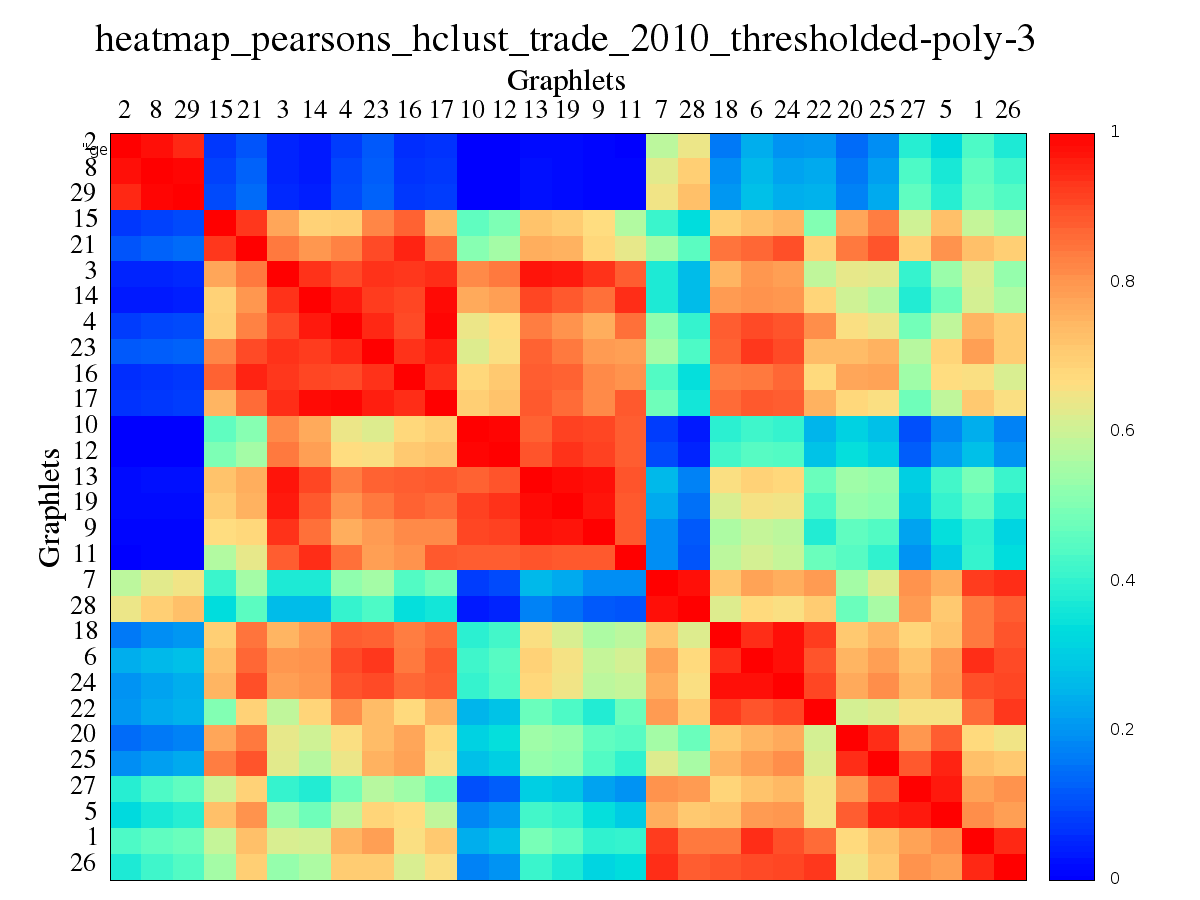
\includegraphics[scale=0.4]
{../code/final_results/trade_2010_thresholded/heatmap_pearsons_hclust_trade_2010_thresholded-poly-3.png}
\caption{}
\label{fig:trade}
\end{figure}

In the trade network, we can observe several clusters of graphlets that ahave been formed along the diagonal:
\begin{itemize}
 \item Cliques cluster made of graphlets 2,8,29. If a country has a lot of cliques in its neighbourhood, then it is part of a densely connected group of countries. 
 \item A cluster that is made of graphlets 15,21,3,14,4,23,16,17,10,12,13,19,9 
 and 11 which can be split into 2 further sub-clusters: 
    \begin{itemize}
     \item P4 cluster made of graphlets 15,21,3,14,4,23,16,17. These are all 
     graphlets that contain a P4 (path on 4 nodes, graphlet G3). 
     \item Claw cluster made of 10,12,13,19,9,11. These graphlets all contain C3 ( claw on 3 nodes, graphlet G4)
    \end{itemize}
\end{itemize}

\textbf{It should be noted that the diameter of the trade network is really small (aprox 5). This means that nodes will share a large proportion of their neighbourhood, especially hub nodes. In order to fix this issue, we have tried to threshold the economic networks at a level lower than 85\% in order to remove some of the edges and thus yield a higher diameter. However, this has not resulted in a lower diameter (it stayed constant at around 5), which meant that our metric might not be suitable for analysing this type of networks.}

\section*{Trade network over the years}

\subsection*{1962 to 1972}

\begin{figure}[H]
  \centering
  \label{fig:asafa}
  
  \subfloat{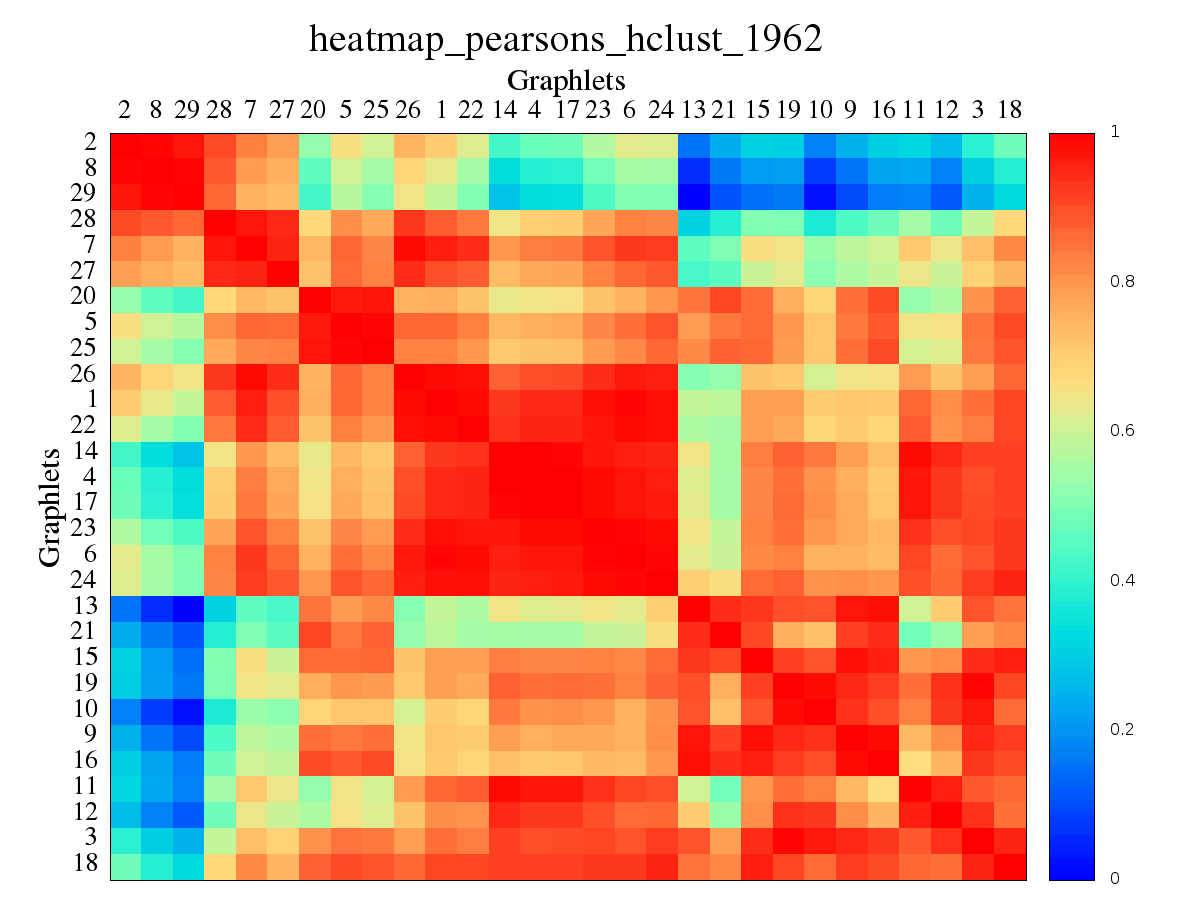
\includegraphics[width=70mm]{../code/final_results/all_trade_thresh/heatmap_pearsons_hclust_1962.png}}
  \subfloat{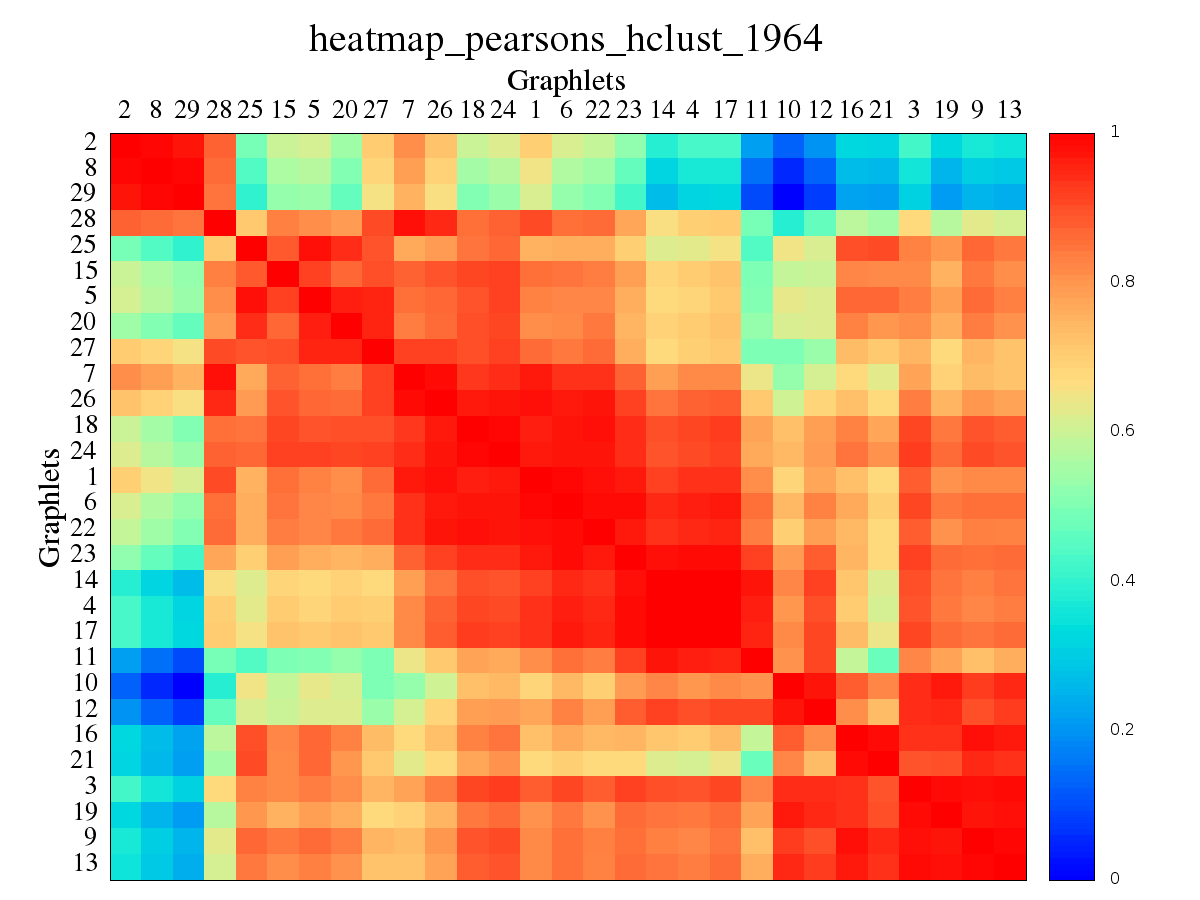
\includegraphics[width=70mm]{../code/final_results/all_trade_thresh/heatmap_pearsons_hclust_1964.png}}
  \\
  \subfloat{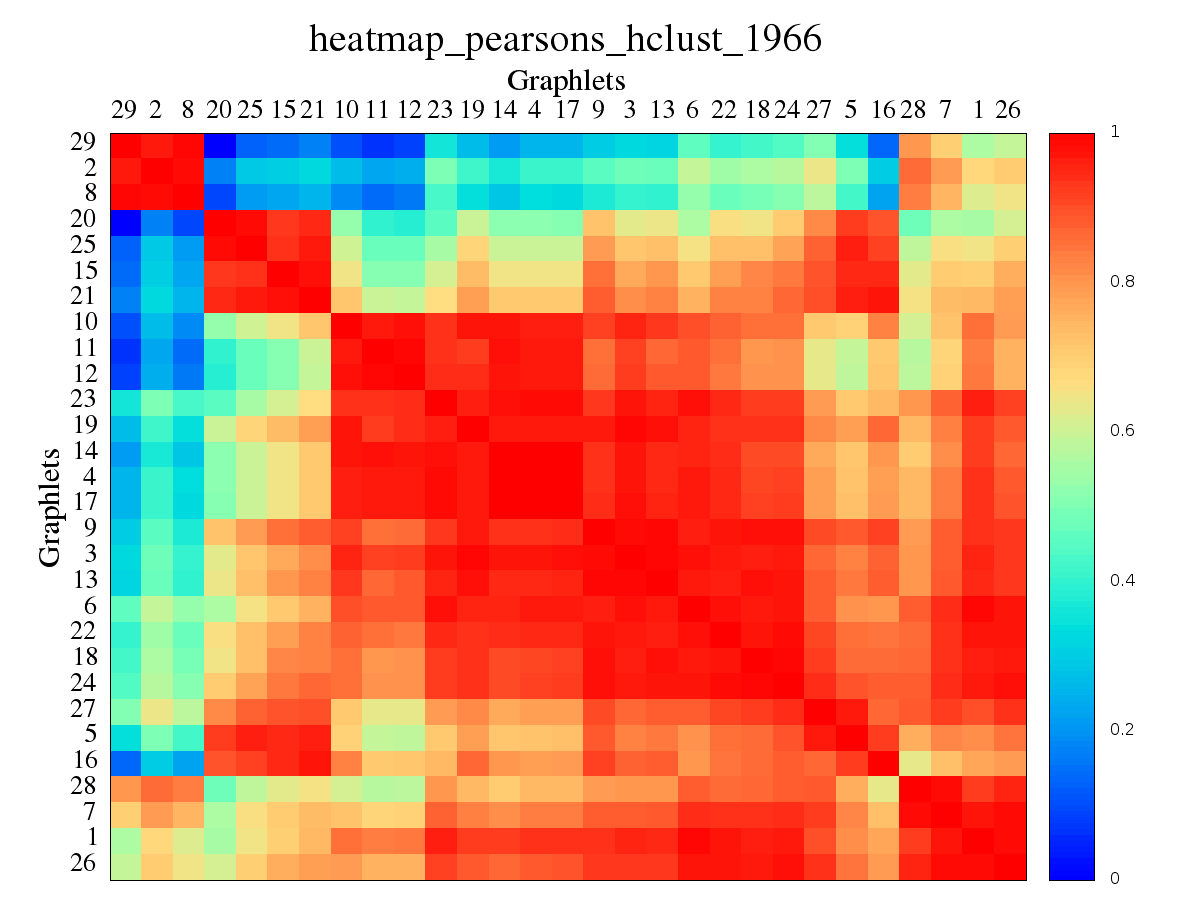
\includegraphics[width=70mm]{../code/final_results/all_trade_thresh/heatmap_pearsons_hclust_1966.png}}
  \subfloat{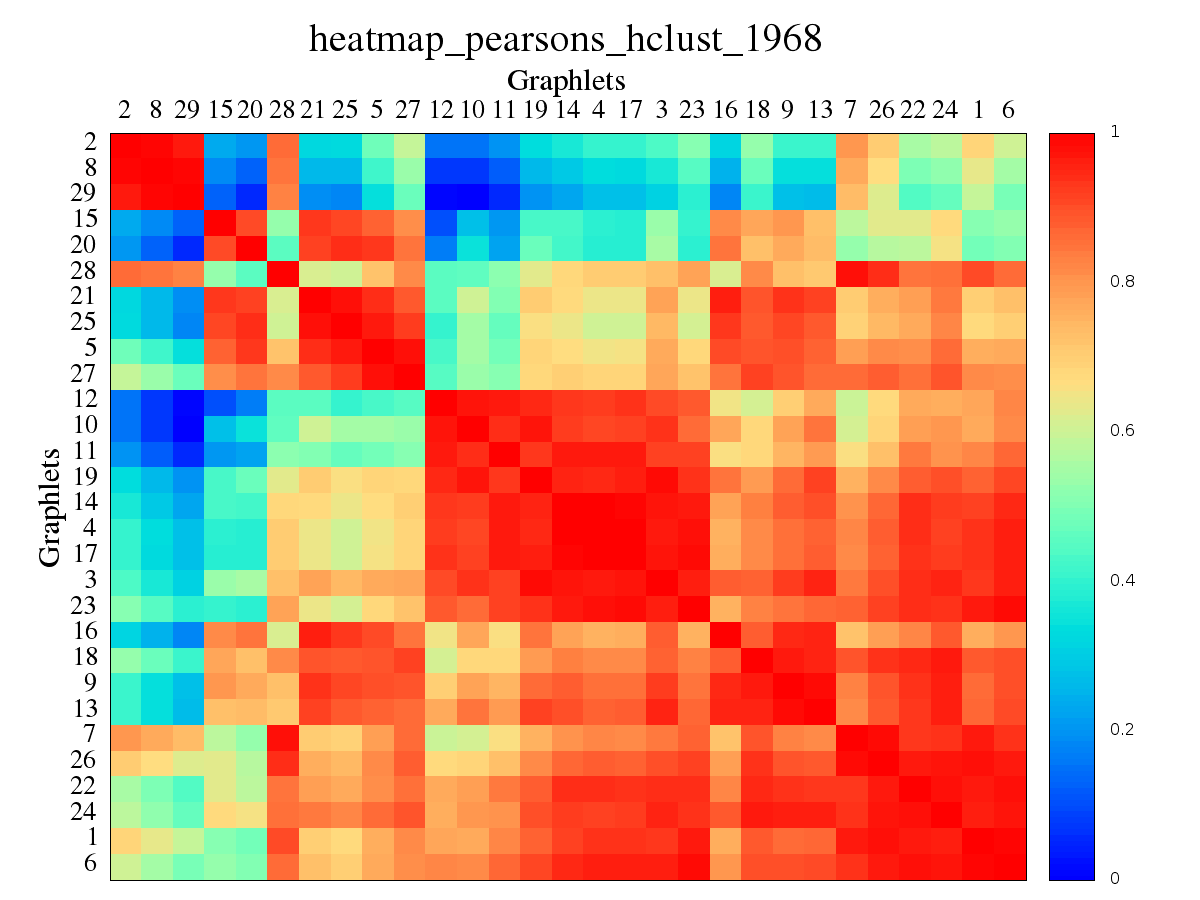
\includegraphics[width=70mm]{../code/final_results/all_trade_thresh/heatmap_pearsons_hclust_1968.png}}
  \\
  \subfloat{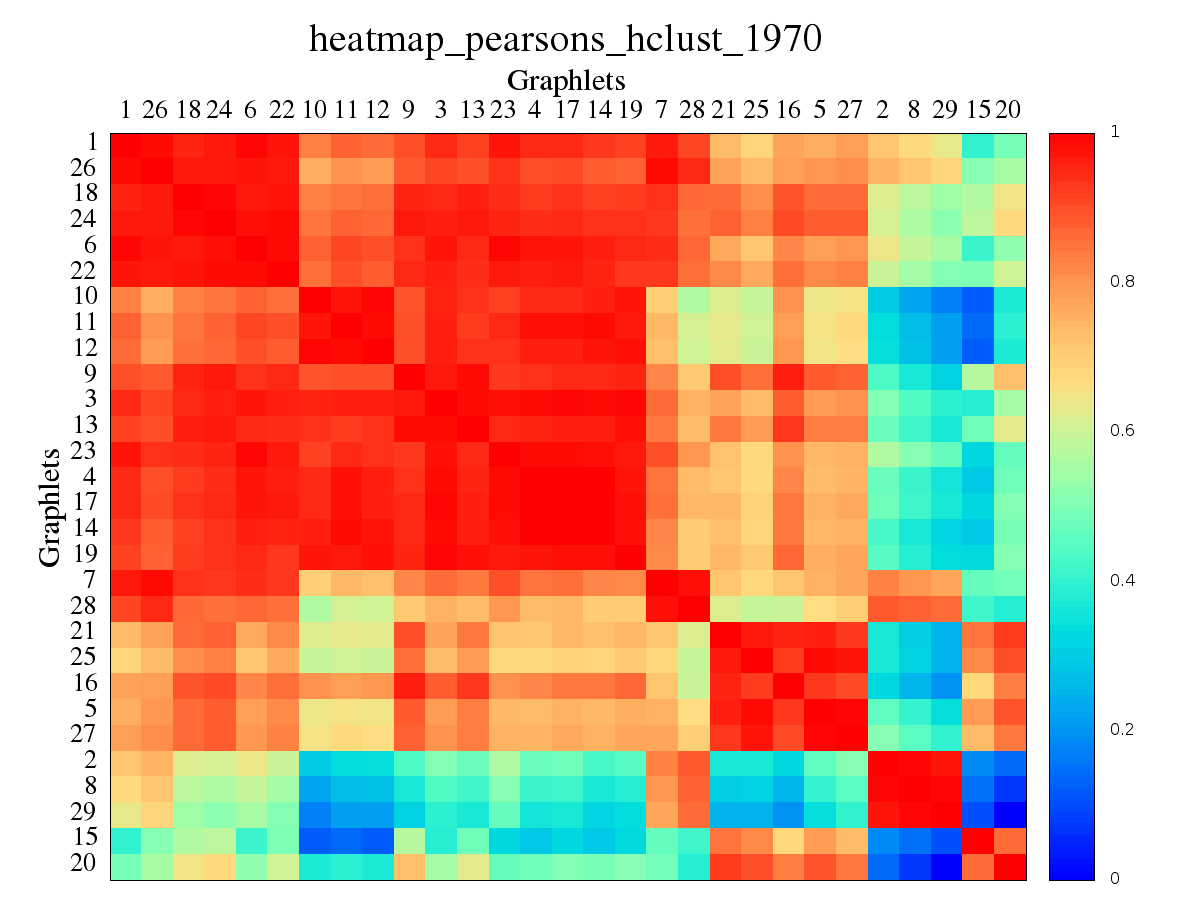
\includegraphics[width=70mm]{../code/final_results/all_trade_thresh/heatmap_pearsons_hclust_1970.png}}
  \subfloat{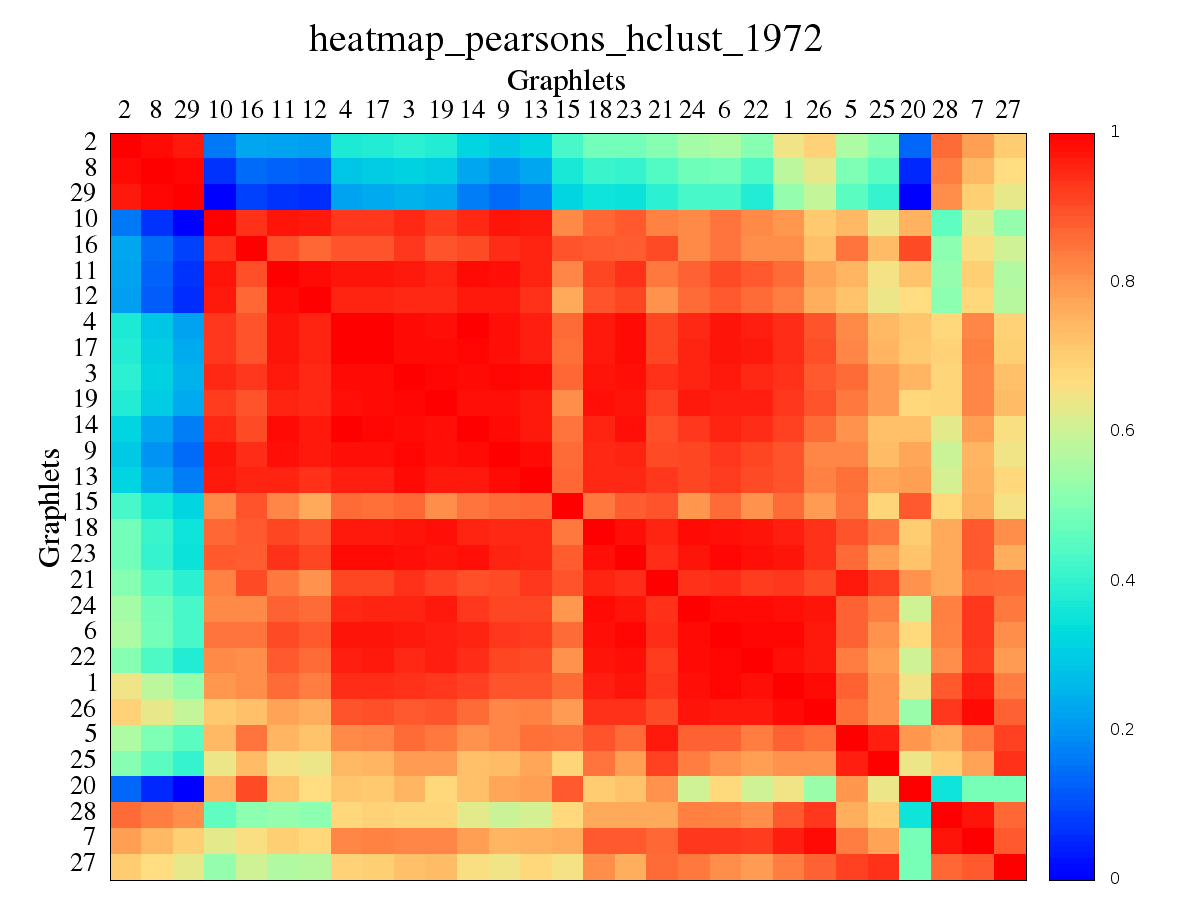
\includegraphics[width=70mm]{../code/final_results/all_trade_thresh/heatmap_pearsons_hclust_1972.png}}

\end{figure}

The first thing we notice is that the cliques 2,8 and 29 cluster together in each 
of the years analysed. In most of the years (apart from 1972) we also observe a 
cluster containing Graphlets that are made of cycles of length 4 (graphlet G5), 
with proeminent graphlets including 5, 20, 21 and 25. 

Another trend we notice is that the graphlets become more and more correlated 
(this will be even more obvious in the second batch of years 1974-1984). This 
might be an effect of globalization, as countries become more and more connected 
and the diameter of the trade network gets smaller. This in turn causes the 
countries to have share a higher proportion of the neighbourhood, which yields 
a higher graphlet correlation.




\subsection*{1974 to 1984}

\begin{figure}[H]
  \centering
  \label{fig:asafa}
  
  \subfloat{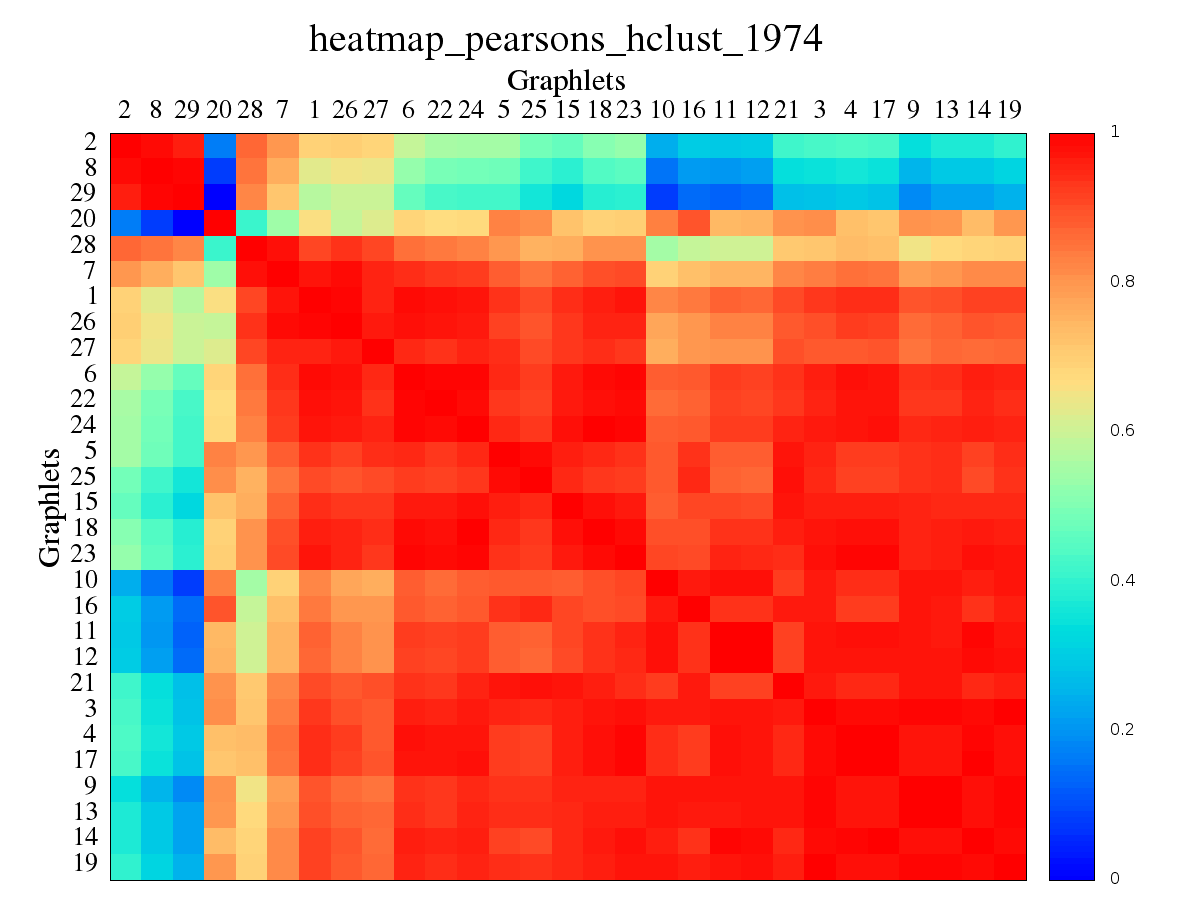
\includegraphics[width=70mm]{../code/final_results/all_trade_thresh/heatmap_pearsons_hclust_1974.png}}
  \subfloat{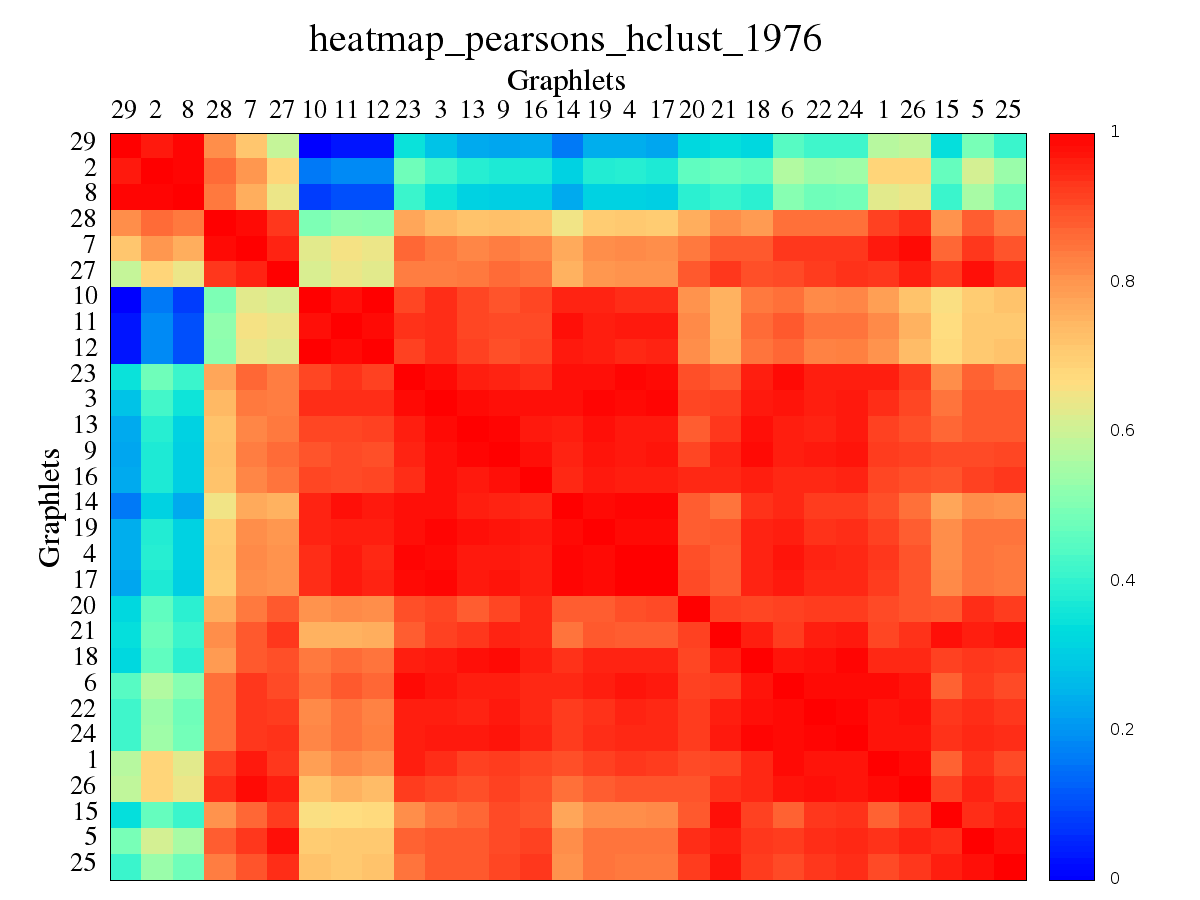
\includegraphics[width=70mm]{../code/final_results/all_trade_thresh/heatmap_pearsons_hclust_1976.png}}
  \\
  \subfloat{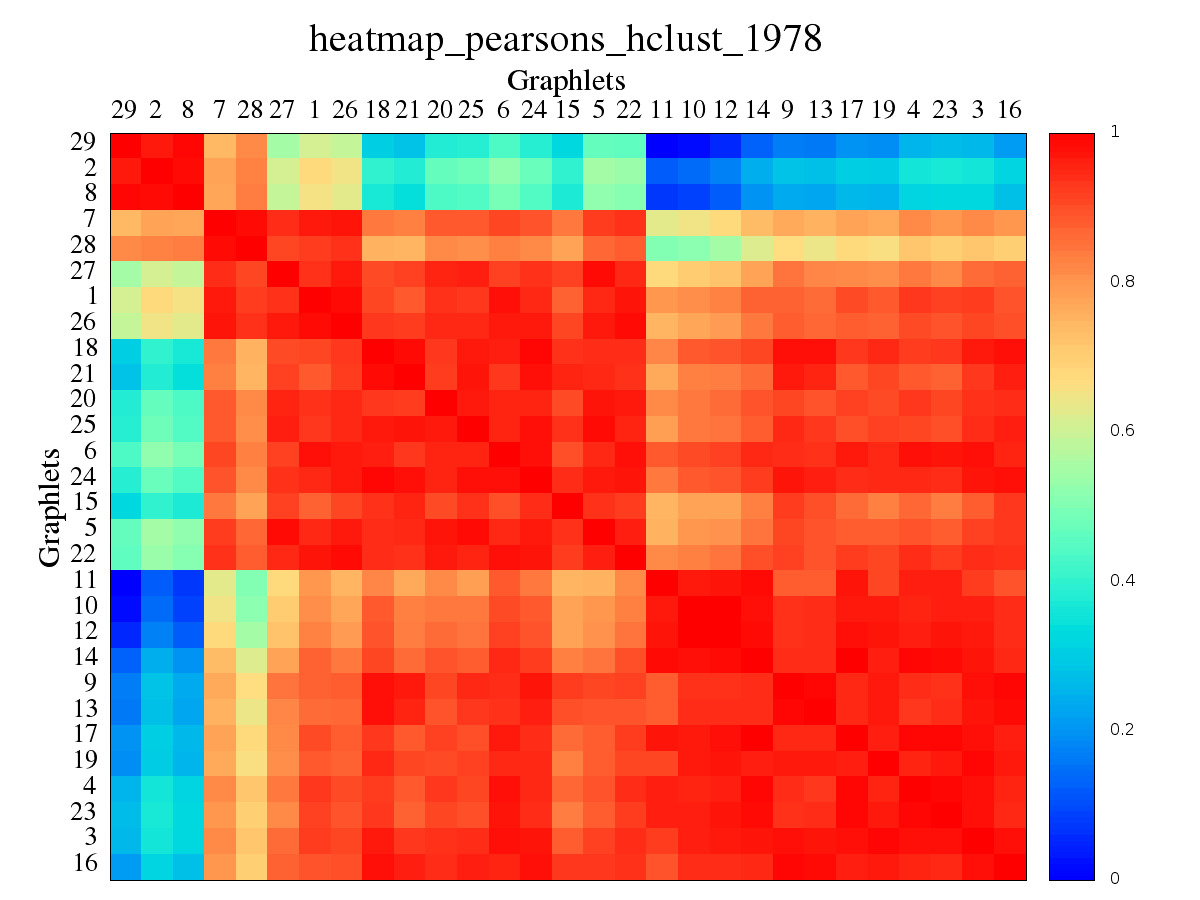
\includegraphics[width=70mm]{../code/final_results/all_trade_thresh/heatmap_pearsons_hclust_1978.png}}
  \subfloat{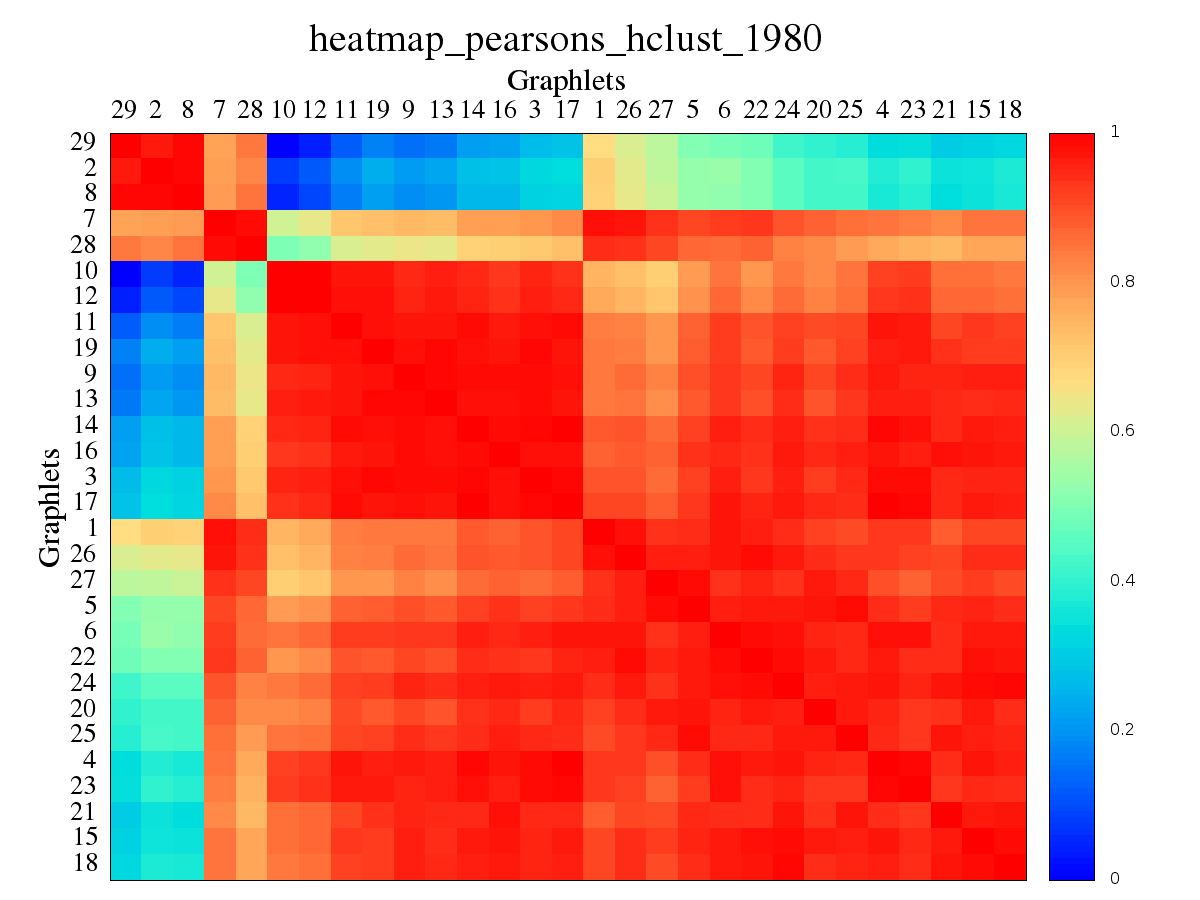
\includegraphics[width=70mm]{../code/final_results/all_trade_thresh/heatmap_pearsons_hclust_1980.png}}
  \\
  \subfloat{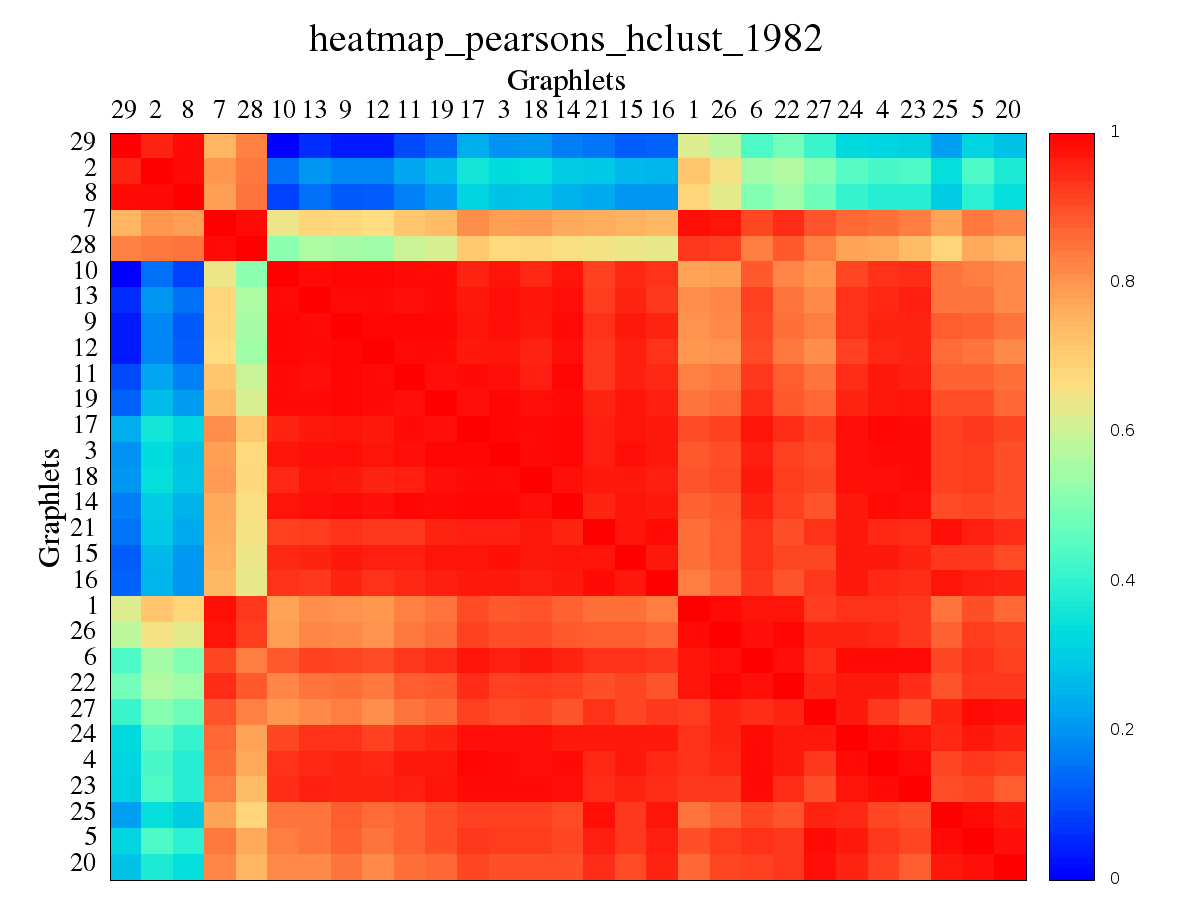
\includegraphics[width=70mm]{../code/final_results/all_trade_thresh/heatmap_pearsons_hclust_1982.png}}
  \subfloat{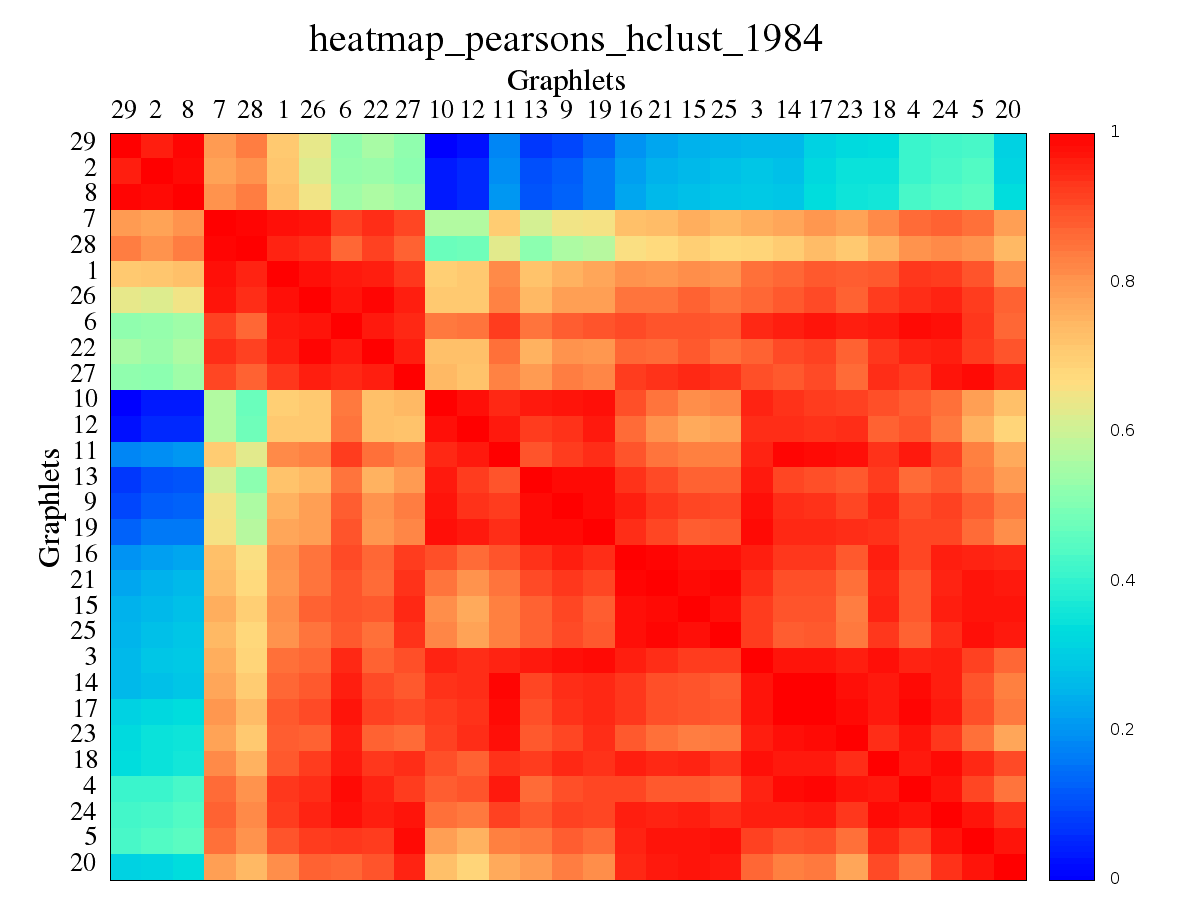
\includegraphics[width=70mm]{../code/final_results/all_trade_thresh/heatmap_pearsons_hclust_1984.png}}

\end{figure}

We also observe that the cliques 2,8 and 29 cluster together in every year 
that has been analysed in this period. In year 1980 we also observe  a cluster 
that is made of graphlets 10,12,11,19,9,13,14,16,3 and 17. All of these 
contain P4's (paths of length 4, graphlet G3). This cluster on P4 can also be 
observed in years 1976 and 1982, but the order in which graphlets appear is 
different, due to the clustering algorithm.

In year 1984, we can actually notice several small clusters on the diagonal. 
One cluster is made of graphlets 7, 28, 1, 26, 6, 22 and 27, which all have a 
P3 (path on 3 nodes, grahplet G1). However, cluster 10,12,11,13,9,19 is 
made of graphlets that don't seem to have a lot in common apart from P2's. 
Cluster 16,21,15 and 25 is mostly made of graphlets that have cycles of length 
4, apart from graphlet G15 which has a cycle of length 5.

On broad terms, we also notice that the graphlets become much more correlated 
in this period, as a result of globalisation. 

\subsection*{1986 to 1996}

\begin{figure}[H]
  \centering
  \label{fig:asafa}
  
  \subfloat{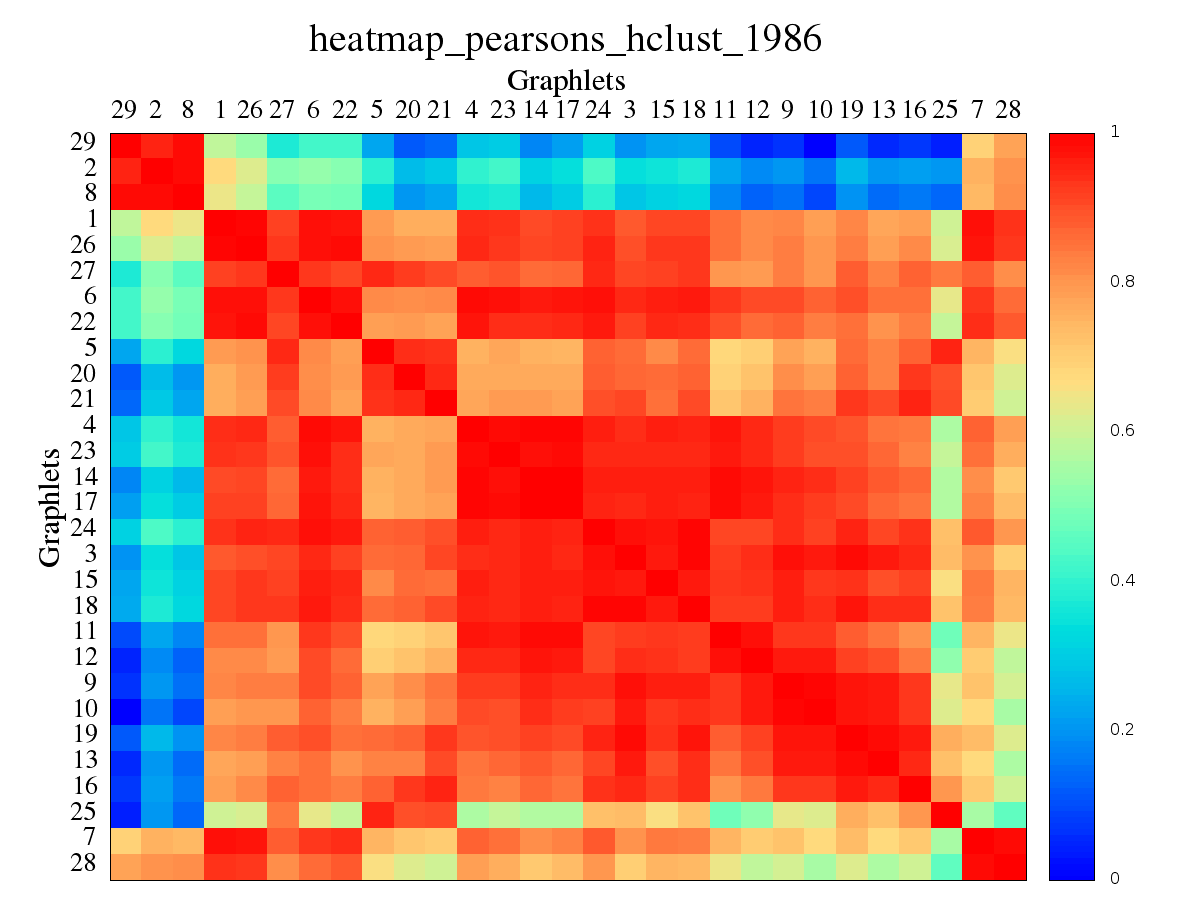
\includegraphics[width=70mm]{../code/final_results/all_trade_thresh/heatmap_pearsons_hclust_1986.png}}
  \subfloat{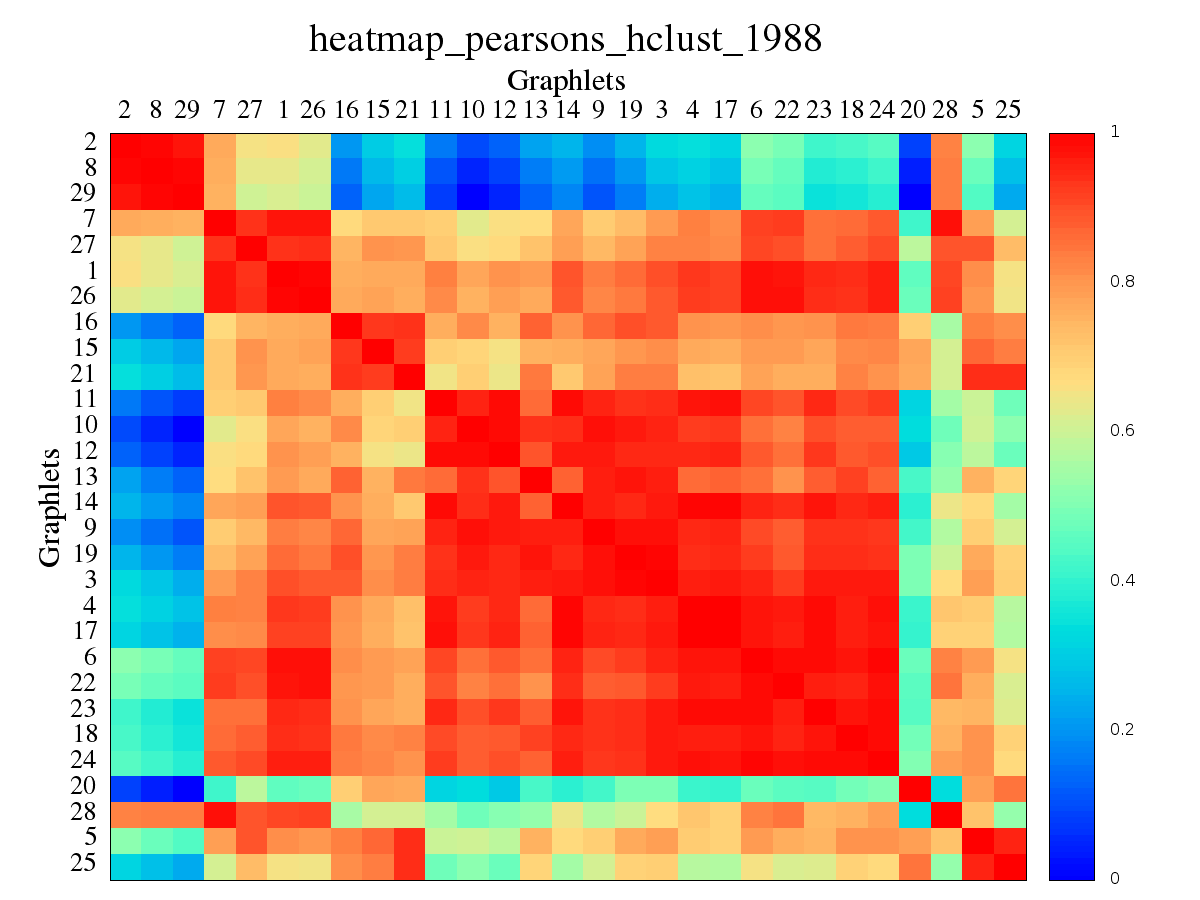
\includegraphics[width=70mm]{../code/final_results/all_trade_thresh/heatmap_pearsons_hclust_1988.png}}
  \\
  \subfloat{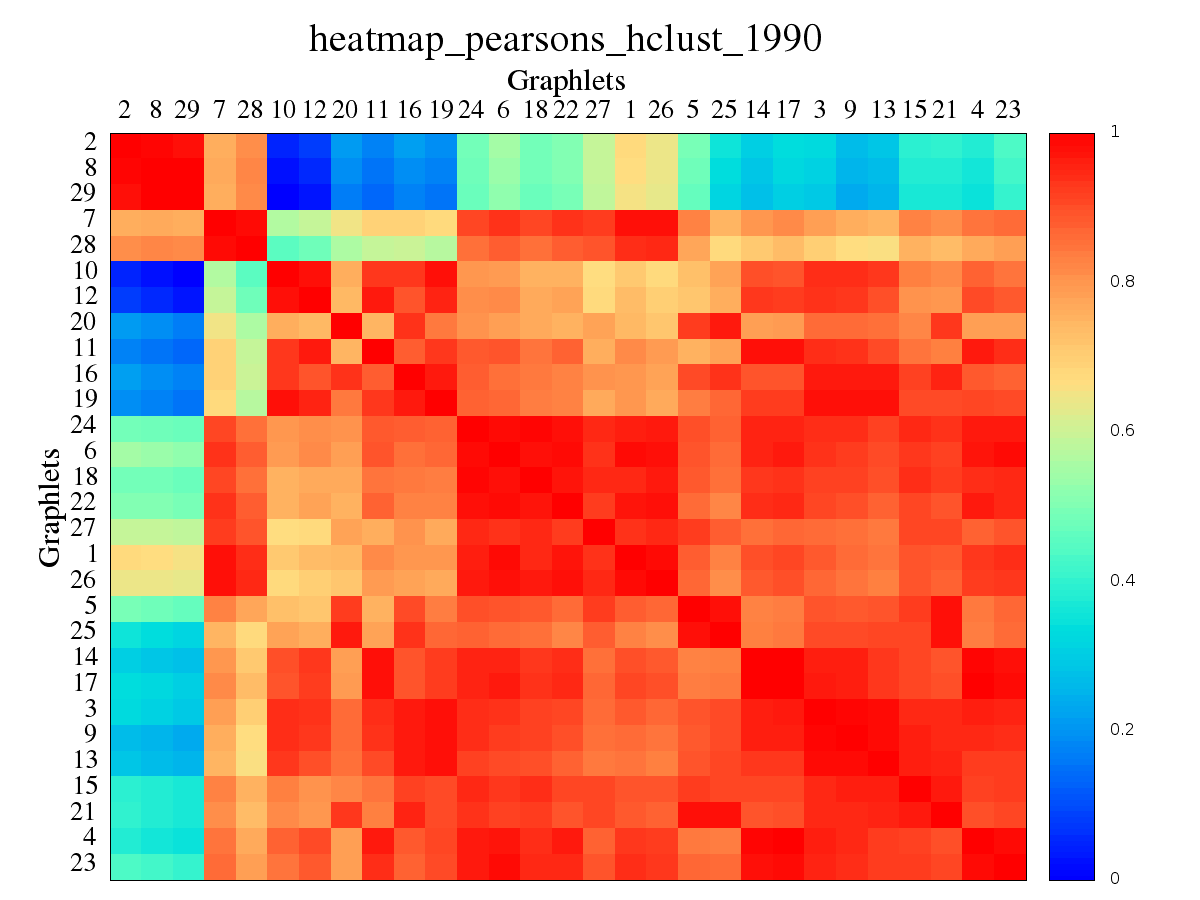
\includegraphics[width=70mm]{../code/final_results/all_trade_thresh/heatmap_pearsons_hclust_1990.png}}
  \subfloat{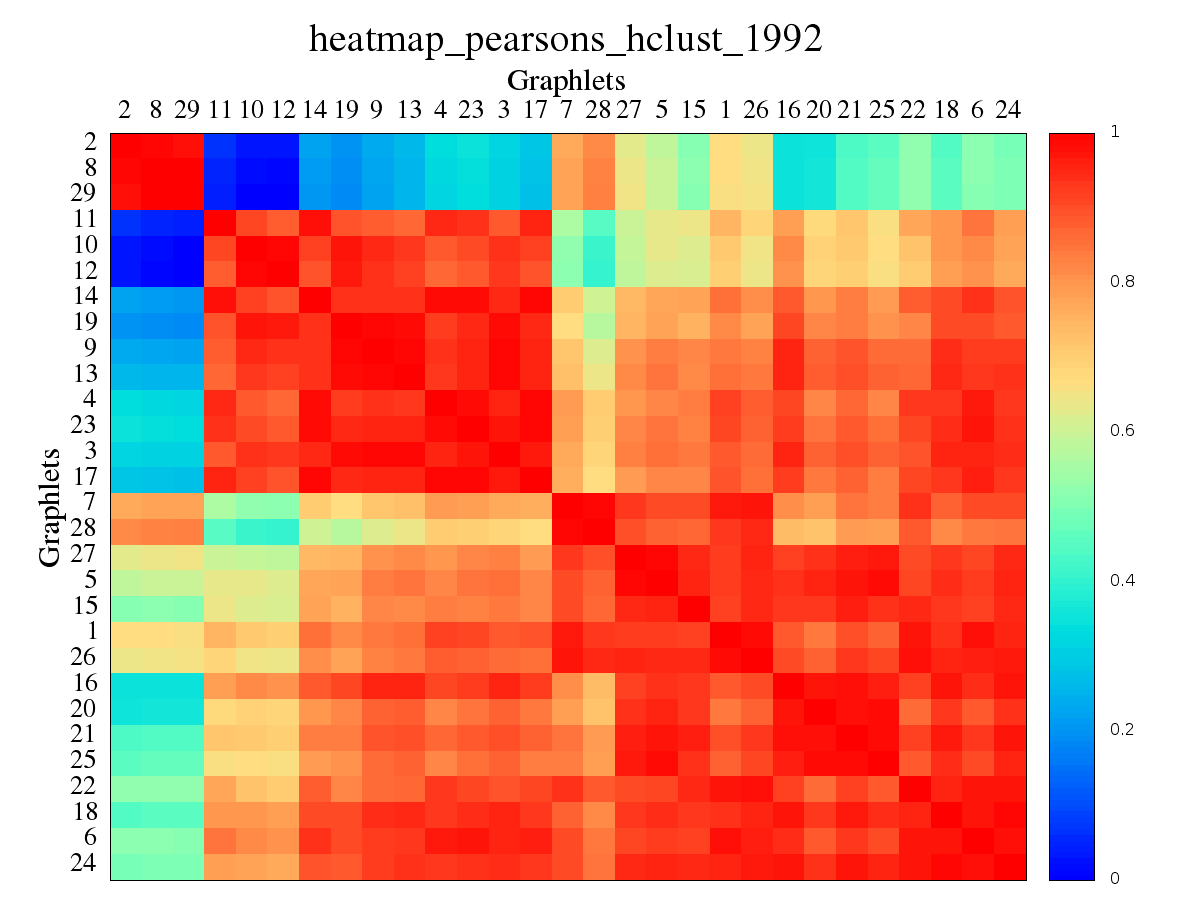
\includegraphics[width=70mm]{../code/final_results/all_trade_thresh/heatmap_pearsons_hclust_1992.png}}
  \\
  \subfloat{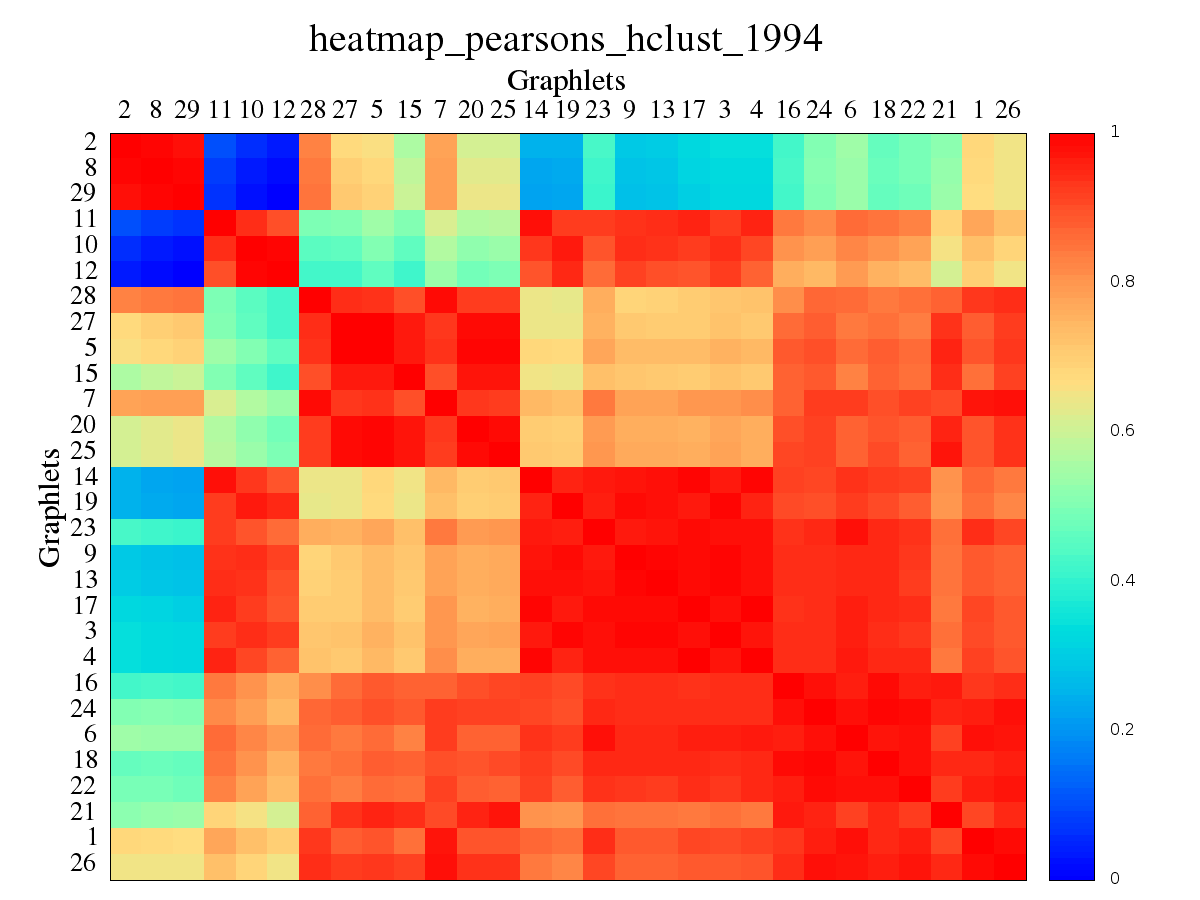
\includegraphics[width=70mm]{../code/final_results/all_trade_thresh/heatmap_pearsons_hclust_1994.png}}
  \subfloat{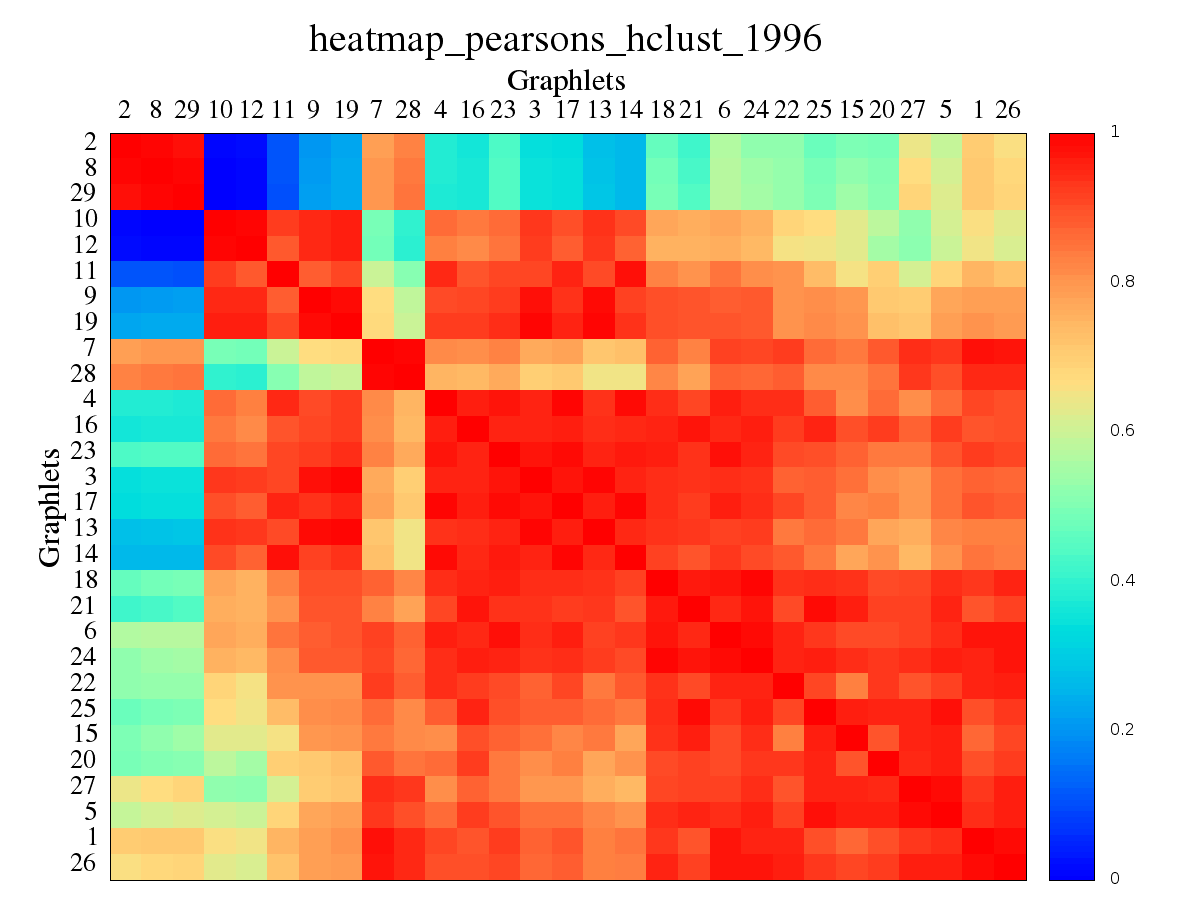
\includegraphics[width=70mm]{../code/final_results/all_trade_thresh/heatmap_pearsons_hclust_1996.png}}

\end{figure}



\appendix
% these do NOT count as part of the suggested page count
% This is probably a good place to explain the models in some detail for example


\subsection*{Trade 1980 - 2010 - CCA results}


\begin{tabular}{ c | l }
p-value (asymptotic Wilks): & 0\\
canonical correlation &  0.895952852603906\\
\hline
"OPENK" & 0.247451850129221\\
"BCA" & 0.200192036020745\\
"KG" & 0.174218020898056\\
"BCAperRGDPL" & 0.147747854581897\\
"KI" & 0.0599886767878585\\
"KC" & -0.0978003022187681\\
"XRAT" & -0.119986658349081\\
"KIxRGDPL" & -0.178691495415784\\
... & ...\\
"KIxRGDPLxPOP" & -0.725521757848721\\
"LE" & -0.758181971837348\\
"POP" & -0.766671415171843\\
\hline
"sig20" & -0.444543442451426\\
"sig15" & -0.575462152591753\\
"sig16" & -0.622031342349607\\
"sig25" & -0.637543533431093\\
"sig5" & -0.661423872853069\\
"sig21" & -0.671415246677959\\
"sig29" & -0.687274648254906\\
"sig27" & -0.708988660894554\\
"sig9" & -0.724239423011173\\
"sig10" & -0.729146326429808\\
"sig11" & -0.733689565547564\\
"sig12"& -0.74053482689155\\
"sig18"& -0.740560758746925\\
"sig28" &-0.745247161501011\\
"sig19"& -0.745807180169319\\
"sig13"& -0.748570010957501\\
"sig8" &-0.750204285105424\\
"sig26"& -0.75733747539876\\
"sig14"& -0.76293066951543\\
"sig24"& -0.764579123039903\\
"sig23"& -0.766556828645173\\
"sig22"& -0.767812484500584\\
"sig17"& -0.778130620463604\\
"sig4" &-0.782701582920566\\
"sig3" & -0.783606882407559\\
"sig7" & -0.793649835514637\\
"sig6" & -0.803147167225324\\
\textbf{"sig2"} & -0.805688869837944\\
"sig1" & -0.823315620830077\\
\end{tabular}\\


CCA results clearly show that big and rich countries that have a high population and GDP per capita have a clustered set of trading partners, while small and poor countries with account deficits have a sparser neighbourhood. The population of the country seems to be quite an important factor for determining whether it will have a neighbourhood rich in graphlets because of the following two reasons:
\begin{itemize}
 \item In the indicators vector, population has the weight with the highest magnitude: 0.766
 \item Most of the other indicators that have a high weight are obtained by mutiplying population with other indicators. It should be noted that this is the case also in Omer et al's paper "Revealing the hidden language" ...
\end{itemize}


\subsection*{Canonical correlation analysis on Economic Integration}

I have tried to analayse whether the level of \emph{Economic Integration} of a country is positively correlated with dense graphlets and negatively correlated with sparse graphlets. This is something to be expected, since when a country is part of a strong trading bloc, then it's neighbours have a higher probability of doing heavy trade with one another. This is because there is incentive for the country to trade more with the partners from the same bloc. This would in turn result in denser graphlets in the neighbourhood of that country. 

I have therefore annotated each country with a number (1-6) that measures the degree of economic integration:
\begin{itemize}
 \item 0 - no economic integration 
 \item 1 - Multilateral Free Trade Area (AFTA, CEFTA, CISFTA, COMESA, GAFTA, GCC
 \item 2 - Customs union (CAN, CUBKR, EAC, EUCU, MERCOSUR, SACU)
 \item 3 - Common market (EEA, EFTA, CES) 
 \item 4 - Customs and Monetary Union (CEMAC/franc, UEMOA/franc) 
 \item 5 - Economic union (CSME, EU) 
 \item 6 - Economic and monetary union (CSME/EC dollar, EU euro)
\end{itemize}


\begin{tabular}{ c | l }
canonical correlation &  0.618823452163313\\
p-value (asymptotic Wilks): & 0.0128012383082338\\
\hline
"Integration" & 0.618823452346073\\
\hline
\textbf{"sig29"} & 0.287035191288073\\
\textbf{"sig8"} & 0.283489421651237\\
\textbf{"sig2"} & 0.278615840865378\\
"sig22" & 0.26819674644438\\
"sig28" & 0.268059123234175\\
"sig7" & 0.260207030053052\\
"sig26" & 0.260112720674704\\
"sig18" & 0.246614831141233\\
"sig1" & 0.238368565474503\\
"sig24" & 0.231333551025451\\
"sig6" & 0.229690387810875\\
"sig4" & 0.220206855982917\\
"sig27" & 0.220129084450554\\
"sig17" & 0.210208580507573\\
"sig14" & 0.206306944610344\\
"sig23" & 0.204204021795578\\
"sig5" & 0.201486106029494\\
"sig20" & 0.193906989388751\\
"sig25" & 0.191223668928417\\
"sig21" & 0.190762668949242\\
"sig16" & 0.190257968164896\\
"sig11" & 0.183299329835195\\
"sig3"& 0.177301380839247\\
"sig15"& 0.168139476991408\\
"sig13"& 0.16763975453569\\
"sig19"& 0.160509773821264\\
"sig9" &0.150872182634174\\
"sig12"& 0.148861465107402\\
"sig10"& 0.146375591601729\\
\end{tabular}\\

The CCA analysis of Economic integration clearly shows that dense graphlets such as cliques {29,8,2} are most correlated with the level of economic integration. At the other end of the spectrum we have much sparser graphs, such as {10,12,9} that have few edges. This means that countries that are more integrated with their trading partners tend to trade in one cluster (since ), while countries that are less integrated tend to trade with countries that are more separated with each other. 

This could be easily explained in economic terms, because if the trading partners of other countries form a highly connected cluster, then that country has more incentives to become integrated with its partners. The reverse effect also holds: when a country becomes more integrated within a trading bloc, a considerable ammount of its trade tends to shift to within the trading bloc. For example, this has been the case with countries that joined the EU in 1992 (Austria, Sweeden and Finland) and 2004(Czech Republic, Poland, Hungary, etc ..). 

\subsection*{Change over years}

\begin{figure}[H]
  \centering
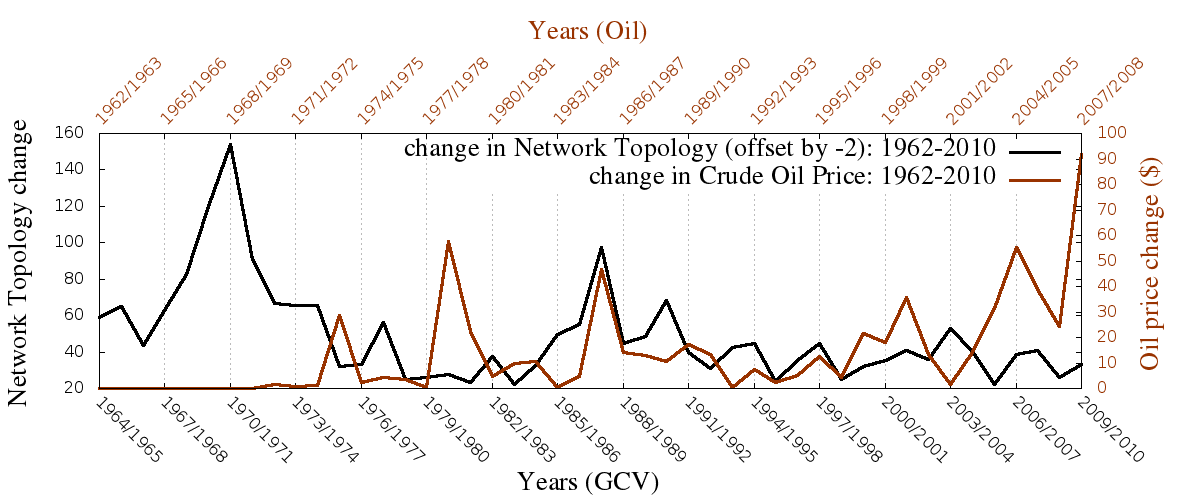
\includegraphics[scale=0.4]
{../code/final_results/all_trade_thresh/change_over_time.png}
\caption{}
\label{fig:hsa_meta}
\end{figure}

Important economic events that match the graph:
\begin{itemize}
 \item Black Monday of 1987
 \item OPEC oil crisis 1973 (although the peak in our graph occurs 3 years earlier)
 \item 1990's revolutions in Eastern Europe that mark a starting point of 
 increasing trade between Western Europe and Eastern Europe
 \item Arab Spring Revolts
\end{itemize}


\subsection*{Food and live animals - CCA results}


\begin{tabular}{ c | l }
canonical correlation &  0.954399648341325\\
\hline
"BCA" & 0.547689925367287\\
"BCAperRGDPL" & 0.500823424204372\\
"OPENK" & 0.243606879775848\\
"KI" & 0.209884267951759\\
... & ...\\
"KCxRGDPL" & -0.420546719870103\\
"KIxRGDPLxPOP" & -0.871656464696992\\
"LE" & -0.877434636132884\\
"POP" & -0.881642665100747\\
"KGxRGDPLxPOP" & -0.902330822089951\\
"RGDPLxPOP" & -0.911676654572702\\
"RGDPCHxPOP" & -0.911684561314991\\
"RGDPL2xPOP" & -0.911764842878327\\
"KCxRGDPLxPOP" & -0.914794036209158\\
\hline
"sig29"  & -0.671790063754862\\
"sig8" & -0.713976480166582\\
... & ...\\
"sig3" & -0.889319524129654\\
"sig19" & -0.892822123308914\\
"sig13" & -0.896528616555174\\
\end{tabular}\\


\subsection*{Minerals and fuels - CCA results}

Similar results as for food and live animals.


\section*{Conclusion}  
  To conclude, we can clearly say that the main reason for the graphlets clustering together is because they contain as subgraphs the same smaller graphlets. Moreover, the CCA analysis that has been performed on several metabolic, ppi and trade networks has not been able to clearly separate the graphlets into sets with positive and negative weights. The best CCA correlations have been obtained with the trade network (~0.9), followed by some Yeast PPI networks (~0.5) and compounds-based metabolic networks (~0.5). This means that a high correlation (around 90\%) between economic indicators and graphlet GCV signatures can be achieved in the trade network. The reason for the high correlation in the trade network might come as a result of the small size and diameter in this network (119 nodes). 
  
  For the yeast ppi networks, a correlation of around 0.5 indicates that there is some connection between the GCV signature and the 
  ppi annotations. The reason for this might be because the GCV signature only captures some information about the neighbourhood of the protein. Moreover, other differences between proteins might not be due to the way they interact with the environment, but due to their chemical and physical properties.
  

\end{document}
